\documentclass{beamer}
%INTRODUZIONE PACCHETTI
\usepackage[british,UKenglish,USenglish,english,american]{babel}
\usepackage[utf8]{inputenc}
\usepackage[T1]{fontenc}
\usepackage[tight]{minitoc}
\usepackage{mathtools}
\usepackage{xcolor}
\definecolor{dgreen}{rgb}{0.,0.6,0.}
\usepackage{amsmath}
\usepackage{amssymb}
\usepackage{amsthm}
\usepackage{mathrsfs}

% package and commands for algorithms
\usepackage{algorithm,algcompatible,algpseudocode}
\algnewcommand\INPUT{\item[\textbf{Input:}]}%
\algnewcommand\OUTPUT{\item[\textbf{Output:}]}%

%DEFINIZIONE COSE
\title{Frank-Wolfe for White Box Adversarial Attacks}
\subtitle{\normalsize Department of Mathematics "Tullio Levi-Civita"\\
Master's Degree in Data Science}
\author[Greta Farnea]{\large Eleonora Brasola \\ Alberto Cocco \\ Greta Farnea}
\date{\vspace{.5cm} \;}
\institute[]{Università di Padova}

%DEFINIZIONE STILI TH/PROP ... 
\usetheme{Padova}
\setbeamercovered{dynamic}
\usepackage[style=alphabetic,backend=bibtex]{biblatex}
\usepackage{multimedia}
% italian versions ***************************** 
%\theoremstyle{plain}
%\newtheorem{thm}{Teorema}[section]
%\newtheorem{lem}{Lemma}[section]
%\newtheorem{prop}{Proposizione}[section]
%\theoremstyle{definition}
%\newtheorem{defn}{Definizione}[section]
% english versions ***************************** 
\theoremstyle{plain}
\newtheorem{thm}{Theorem}[section]
\newtheorem{lem}{Lemma}[section]
\newtheorem{prop}{Proposition}[section]
\theoremstyle{definition}
\newtheorem{defn}{Definition}[section]



%Definisco argmax/argmin come unico operatore 
\DeclareMathOperator*{\argmax}{arg\,max}
\DeclareMathOperator*{\argmin}{arg\,min}

\newcommand\blfootnote[1]{%
  \begingroup
  \renewcommand\thefootnote{}\footnote{#1}%
  \addtocounter{footnote}{-1}%
  \endgroup
}

%**********************************************************************************

\begin{document}
%SLIDE 1: TITOLO
\begin{frame}
\maketitle
\end{frame}

\begin{frame}{Introduction to Adversarial attacks}
\textbf{Adversarial example}: element drawn from data distribution that is perturbed with some noise
    \begin{itemize}
            \item \textbf{Misclassification}: distorted image is not properly recognized by the DNN
            \item \textbf{Transferability}: different DNNs misclassify in the same way
    \end{itemize}
\medskip

\begin{columns}
\begin{column}{0.4\textwidth}
\begin{figure}[ht]
  \centering
  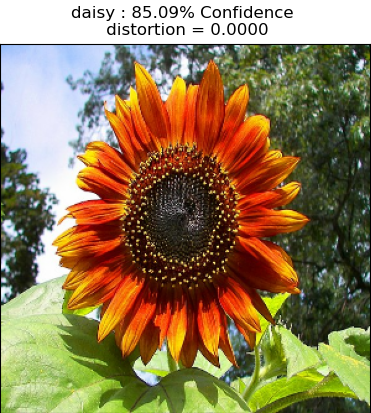
\includegraphics[width=0.7\columnwidth]{Images/original.png}\\
  %\caption{Original image }
\end{figure}
\end{column}
\begin{column}{0.2\textwidth}
$\to$ adding a small noise, the adversarial image fools the DNN $\to$
\end{column}
\begin{column}{0.4\textwidth}
\begin{figure}[ht]
  \centering
  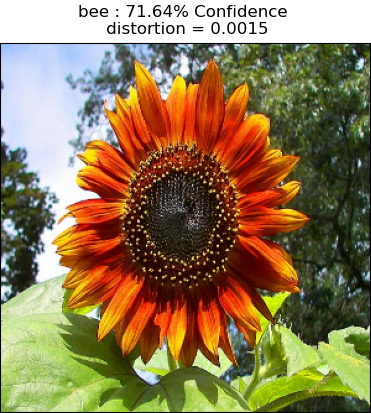
\includegraphics[width=0.7\columnwidth]{Images/fw_untargeted.png}\\
  %\caption{Adversarial image }
\end{figure}
\end{column}
\end{columns}

\blfootnote{Figures obtained from \textit{demo.py}}

\end{frame}

\begin{frame}{Different types of attacks}
We can decide if we want control on the output target of the adversarial image
    \begin{itemize}
        \item \textbf{Untargeted} attacks: just interested in the misclassification 
        \item \textbf{Targeted} attacks: want a specific  class as output 
    \end{itemize} 
\medskip
According to the information we can retrieve from the DNNs, we can have: 
\begin{itemize}
    \item \textbf{White box} attacks: access to all information, also gradients 
    \item \textbf{Black box} attacks: access only to input and output \\$\to$ techniques for gradient estimation 
\end{itemize}
\end{frame}

\begin{frame}{FGSM}
\textbf{Notation: }
\begin{itemize}
    \item  $x_\text{ori}$ : original image
    \item $\ell(\cdot)$: loss function
\end{itemize}

\bigskip
One of the simplest adversarial method and one of first that has been implemented: 
\begin{itemize}
    \item One-step gradient-based method
    \item Maximum distortion $\epsilon$
\end{itemize}
\begin{align*}
    x &= x_\text{ori} + \epsilon \text{sign}(\nabla_x \ell(x_\text{ori}) \qquad \text{(untargeted);} \\
    x &= x_\text{ori} - \epsilon \text{sign}(\nabla_x \ell(x_\text{ori}) \qquad \text{(targeted).}
\end{align*}

\blfootnote{\textit{Explaining and Harnessing Adversarial Examples}, Goodfellow et al. }
    
\end{frame}

\begin{frame}{PGM}

\begin{itemize}
    \item Projection-based iterative approach 
    \item Slow method 
\end{itemize}
    \begin{algorithm}[H]
\caption{PGM}\label{PGD}
\begin{algorithmic}[1]
\For{$k=1 \dots$}
  \State Set $ \bar{x}_k = \rho_C(x_k + s_k \nabla f(x_k))$ \Comment{if untargeted, $s_k > 0$}
  \State Set $ \bar{x}_k = \rho_C(x_k - s_k \nabla f(x_k))$ \Comment{if targeted, $s_k > 0$}
  \State If $\bar{x}_k$ satisfies some specific condition, then STOP
  \State Set $x_{k+1} = x_k + \gamma_k (\bar{x}_k - x_k)$ \Comment{with $\gamma_k \in (0, 1]$}
    
\EndFor
\end{algorithmic}
\end{algorithm}

\blfootnote{\textit{Optimization for Data Science Notes}, Rinaldi}
\end{frame}

\begin{frame}{MI-FGSM}
\begin{itemize}
    \item Iterative version of \textit{FGSM}, adding a momentum term 
    \item High distortion values
\end{itemize}

    \begin{algorithm}[H]
\caption{MI-FGSM}\label{MI_FGSM}
\begin{algorithmic}[1]

\State Fix $g_0 = 0$ and $x_{0}^\ast$ %$\gamma = \epsilon / T$
\For{$t=0$ to $T-1$}
    \State Input $x_t$ and obtain the gradient $\nabla_x f(x_t)$

    \State $
        g_{t+1} = \beta \cdot g_t + \frac{\nabla_x f(x_t)}{\Vert \nabla_x f(x_t) \Vert_1}$
    \State $
        x_{t+1} = x_t + \gamma \cdot \text{sign} (g_{t+1}) $ \Comment{if untargeted}
    \State $x_{t+1} = x_t - \gamma \cdot \text{sign} (g_{t+1}) $ \Comment{if targeted}
    
\EndFor
\end{algorithmic}
\end{algorithm}

\blfootnote{\textit{Boosting Adversarial Attacks with Momentum}, Dong et al.}
\end{frame}


\begin{frame}{FW-white}
\begin{itemize}
    \item Projection-free method with momentum term
    \item Good trade-off between success and distortion 
\end{itemize}
    \begin{algorithm}[H]
\caption{FW-White}\label{FW}
\begin{algorithmic}[1]
\State Set $x_0 = x_{\text{ori}}$, $m_{-1} = - \nabla_x f(x_0)$ if untargeted attack, $m_{-1} = \nabla_x f(x_0)$ if targeted attack
\For{$t=0$ to $T-1$}
    \State $m_t = \beta \cdot m_{t-1} - (1-\beta) \cdot \nabla f(x_t) $ \Comment{if untargeted}
    \State $m_t = \beta \cdot m_{t-1} + (1-\beta) \cdot \nabla f(x_t) $ \Comment{if targeted}
    \State $v_t = \text{argmin}_{x \in C} \langle x, m_t \rangle = - \epsilon \cdot \text{sign} (m_t) + x_{\text{ori}} $
    \State $d_t = v_t - x_t $
    \State $x_{t+1} = x_t + \gamma d_t $
    
\EndFor
\end{algorithmic}
\end{algorithm}

\blfootnote{\textit{A Frank-Wolfe Framework for Efficient and Effective Adversarial Attacks}, Chen et al.}
\end{frame}

\begin{frame}{Demo.py}
    Now we hand over the word to Alberto so that we can see a demo of our project. 
\end{frame}

\end{document}


